% Copyright 2004 by Till Tantau <tantau@users.sourceforge.net>.
%
% In principle, this file can be redistributed and/or modified under
% the terms of the GNU Public License, version 2.
%
% However, this file is supposed to be a template to be modified
% for your own needs. For this reason, if you use this file as a
% template and not specifically distribute it as part of a another
% package/program, I grant the extra permission to freely copy and
% modify this file as you see fit and even to delete this copyright
% notice. 

\documentclass[16pt]{beamer}
\usepackage{caption}
\captionsetup[figure]{labelformat=empty}%

\setcounter{tocdepth}{1}
\setbeamertemplate{footline}[page number]
\setbeamertemplate{navigation symbols}{}
\setbeamertemplate{bibliography item}{}

\newenvironment{wideitemize}{\itemize\addtolength{\itemsep}{10pt}}{\enditemize}

% There are many different themes available for Beamer. 
% http://deic.uab.es/~iblanes/beamer_gallery/index_by_theme.hA comprehensive
% list with examples is given here:tml
% You can uncomment the themes below if you would like to use a different
% one:
%\usetheme{AnnArbor}
%\usetheme{Antibes}
%\usetheme{Bergen}
%\usetheme{Berkeley}
%\usetheme{Berlin}
%\usetheme{Boadilla}
%\usetheme{boxes}
%\usetheme{CambridgeUS}
%\usetheme{Copenhagen}
%\usetheme{Darmstadt}
\usetheme{default}
%\usetheme{Frankfurt}
%\usetheme{Goettingen}
%\usetheme{Hannover}
%\usetheme{Ilmenau}
%\usetheme{JuanLesPins}
%\usetheme{Luebeck}
%\usetheme{Madrid}
%\usetheme{Malmoe}
%\usetheme{Marburg}
%\usetheme{Montpellier}
%\usetheme{PaloAlto}
%\usetheme{Pittsburgh}
%\usetheme{Rochester}
%\usetheme{Singapore}
%\usetheme{Szeged}
%\usetheme{Warsaw}

\title{Describing Images Using Natural Language}

% A subtitle is optional and this may be deleted
\subtitle{}

\author{T.~Dieltjens \and W.~Vekemans}
% - Give the names in the same order as the appear in the paper.
% - Use the \inst{?} command only if the authors have different
%   affiliation.

\institute[Universities of Somewhere and Elsewhere] % (optional, but mostly needed)
{
  \inst{}%
  Department of Computer Science\\
  KULeuven
  }
% - Use the \inst command only if there are several affiliations.
% - Keep it simple, no one is interested in your street address.

\date{11 December 2015}
% - Either use conference name or its abbreviation.
% - Not really informative to the audience, more for people (including
%   yourself) who are reading the slides online

\subject{Theoretical Computer Science}
% This is only inserted into the PDF information catalog. Can be left
% out. 

% If you have a file called "university-logo-filename.xxx", where xxx
% is a graphic format that can be processed by latex or pdflatex,
% resp., then you can add a logo as follows:

% \pgfdeclareimage[height=0.5cm]{university-logo}{university-logo-filename}
% \logo{\pgfuseimage{university-logo}}

% Delete this, if you do not want the table of contents to pop up at
% the beginning of each subsection:
\AtBeginSection[]
{
  \begin{frame}<beamer>{Outline}
    \tableofcontents[currentsection]
  \end{frame}
}

% Let's get started
\begin{document}

\begin{frame}
  \titlepage
\end{frame}

\begin{frame}{Outline}
  \tableofcontents[subsubsectionstyle=hide/hide]
  % You might wish to add the option [pausesections]
\end{frame}

\section{Motivation} %W
\begin{frame}{Motivation}{Why image captioning?}
\begin{wideitemize}
\item connects NLP and CV
\item more than object detection
\item image search
\item visually impaired
\end{wideitemize}
\end{frame}
\section{Objectives} %W
\begin{frame}{Objectives}
\begin{wideitemize}
\item caption unseen images
\item extend existing implementation
\item semantic information
\item improvement?
\begin{figure}[tb]
           \centering
           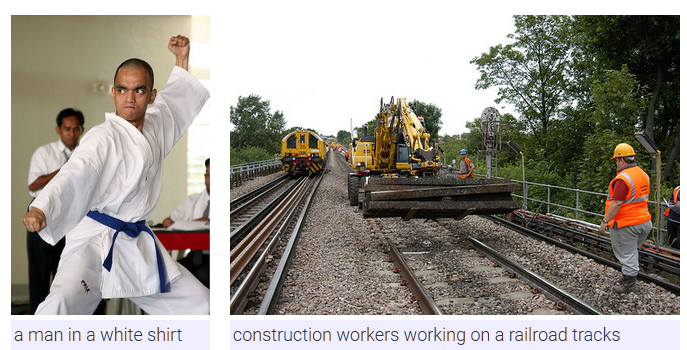
\includegraphics[width=\linewidth]{caption.png}
           \end{figure}
\end{wideitemize}

% ----------------------------------------------------------------------------------

\end{frame}
\section{Background} 
\begin{frame}{Background}
\begin{wideitemize}
\item CNN
\item RNN
\item LSTM
\item LDA
\item Stacked CCA
\end{wideitemize}
\end{frame}

\subsection{CNN}%T
\begin{frame}{Convolutional Neural Networks (CNN)}
\begin{wideitemize}
\item trainable multistage architectures
\item each stage outputs set of arrays called feature map
\item different types of layers
\item faster to train than feed forward
\item unsupervised learning
\item breakthrough in object recognition

\end{wideitemize}
\end{frame}

\begin{frame}{Convolutional Neural Networks (CNN)}
\begin{wideitemize}
\item ImageNet Classification 
\item deeper Models: VGGNet 16 layers
\item use of layers
\begin{figure}[tb]
           \centering
           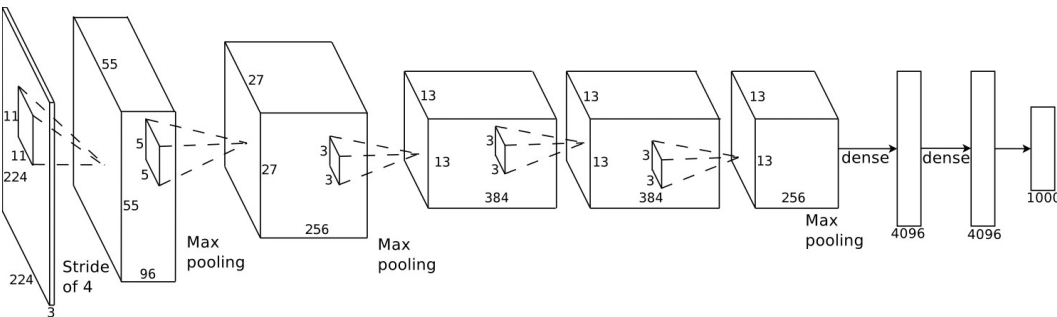
\includegraphics[width=\linewidth]{cnn.PNG}
\\\cite{Krizhevsky2012a}
           \end{figure}

\end{wideitemize}
\end{frame}
\subsection{RNN}%T
\begin{frame}{Recurrent Neural Networks (RNN)}
\begin{wideitemize}
\item predicting sequential data
\item encode temporal information
\item use as language model
\item words represented as word vectors
\begin{figure}[tb]
           \centering
           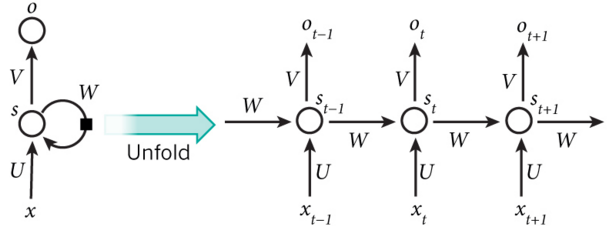
\includegraphics[width=\linewidth]{rnn.PNG}
\\\cite{LeCun2015}
\end{figure}

\end{wideitemize}
\end{frame}

\subsection{LSTM}%T
\begin{frame}{Long Short-Term Memory (LSTM)}{\cite{SeppHochreiter1997}}
\begin{itemize}
\item RNN with memory cells
\item capture long-term dependencies
\begin{figure}[tb]
           \centering
           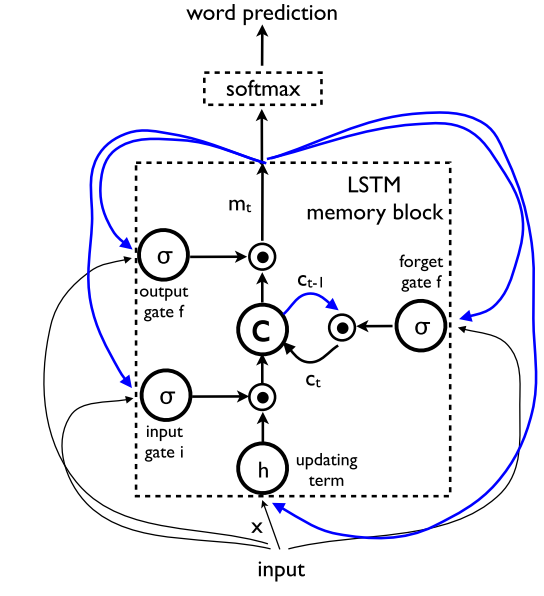
\includegraphics[scale=0.4]{lstm.PNG}
           \\\cite{Google}
\end{figure}

\end{itemize}
\end{frame}



\subsection{LDA}%W
\begin{frame}{LDA \cite{Blei2012}}
\begin{wideitemize}
\item generative probabilistic model for discrete data
\item documents generate topics
\item topics generate words
\item train with e.g. Gibbs sampling

\end{wideitemize}
\end{frame}

\begin{frame}{LDA}
\begin{itemize}
\item $\theta$: per-document topic distribution
\item $z$: topic
\item $w$: word
\end{itemize}
\begin{figure}[tb]
           \centering
           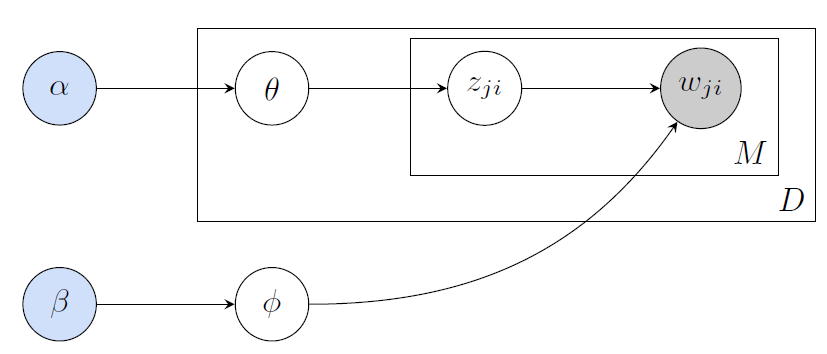
\includegraphics[width=0.6\linewidth]{lda.png}
           \end{figure}
$P(player|doc_i) = P(topic_{sport} | doc_i) P(player | topic_{sport})$

\end{frame}

\subsection{Stacked CCA}%W
\begin{frame}{Stacked CCA \cite{Gong2014}}
\begin{itemize}
\item CCA
    \begin{wideitemize}
    \item canonical correlation analysis
    \item maps two matrices ($A$, $B$) into intermediate representation
    \item maximum correlation between projections of $A$ and $B$ 
    \end{wideitemize}
\item improve embeddings with extra information
\begin{wideitemize}
\item CCA on extra dataset: $A$, $B$
\item $\hat X = [ X, \phi(XA)], \hat Y = [ Y, \phi(YB)]$
\item another CCA on top

% cite Y gong , .....
\end{wideitemize}

\end{itemize}

\end{frame}

% ----------------------------------------------------------------------------------
\section{Related Work}%T
\begin{frame}{Related Work}
\begin{wideitemize}
\item Deep Visual-Semantic Alignments for Genating Image Descriptions \cite{Karpathy2015}
\item Show and Tell: A Neural Image Caption Generator \cite{Google}
\item Guiding Long-Short Term Memory for Image Caption Generation \cite{Fernando2015}
\end{wideitemize}
\end{frame}

\begin{frame}{\cite{Karpathy2015}}
\begin{wideitemize}
\item two goals
\begin{itemize}
\item dense image description based on alignments
\item describing a full image with one sentence 
\end{itemize}
\item alignment model
    \begin{itemize}
    \item Region CNN (RCNN) to detect objects \cite{Girshick2014}
    \item bidirectional RNN to compute word representations
    \item alignment objective
    \end{itemize}
\end{wideitemize}
\end{frame}

\begin{frame}{\cite{Karpathy2015}}
\begin{wideitemize}
\item Multimodal RNN %multimodal staat met hoofdletter in zijn paper
\begin{itemize}
    \item CNN
    \item RNN
    \item Softmax classifier
    \item predicting a sentence with beam search
\end{itemize}
\item Evaluation: 
    \begin{itemize} 
    \item ranking image-sentence retrieval (recall)
    \item sentence predictions (Bleu,METEOR,CIDEr)
    \end{itemize}
\begin{figure}[tb]
           \centering
           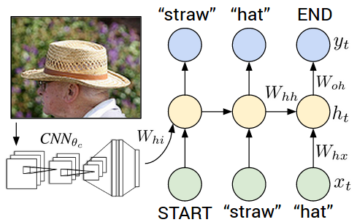
\includegraphics[scale=0.6]{karpathy.PNG}
\end{figure} %TODO referentie


\end{wideitemize}
\end{frame}


\begin{frame}{Neural Image Caption (NIC) \cite{Google}}
\begin{wideitemize}
\item CNN
\item LSTM-based sentence generator
\item train: maximize probability of generating the right caption
\item inference: beam search or sampling
\begin{figure}[tb]
           \centering
           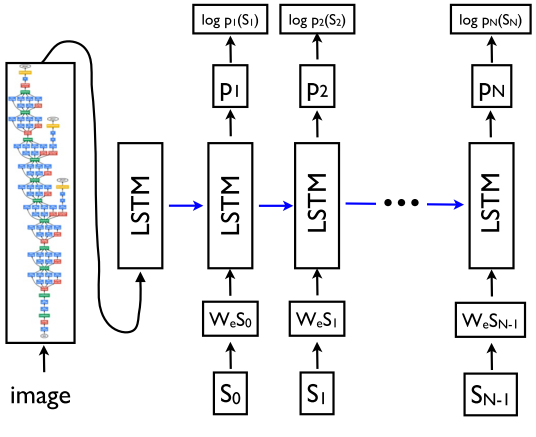
\includegraphics[scale=0.5]{vinyals.PNG}
\end{figure} %TODO referentie

\end{wideitemize}
\end{frame}



\begin{frame}{\cite{Fernando2015}}
\begin{itemize}
\item extension of NIC implementation by Karpathy
\item add semantic information as extra input to LSTM block (guided LSTM)
\begin{itemize}
    \item close sentences
    \item CCA
    \item image
\end{itemize}
\item length normalization strategies for beam search
\end{itemize}
\begin{figure}[tb]
           \centering
           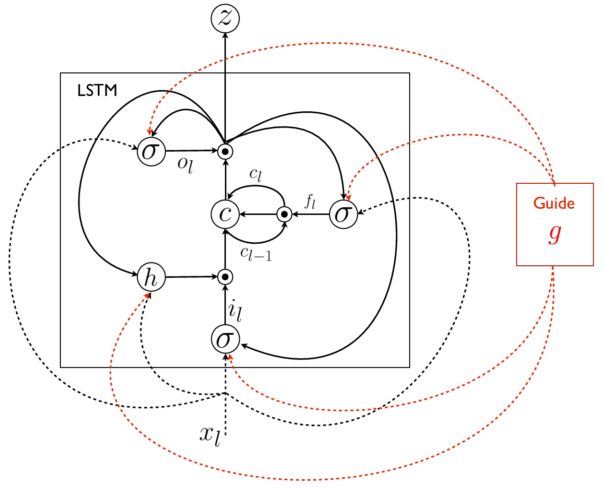
\includegraphics[scale=0.43]{jia.PNG}
\end{figure} %TODO referentie

\end{frame}



% ----------------------------------------------------------------------------------
\section{Datasets}%W
\begin{frame}{Datasets}
\textbf{Manually annotated datasets:}
\begin{itemize}
\item Flickr30k \cite{Young2014}
\begin{itemize}
    \item 31.783 images
    \item 5 captions per image
\end{itemize}
\item MS COCO \cite{Lin2014}
\begin{itemize}
\item Common Objects in COntext
\item over 330.000 images
\item 5 captions per image
\item non-iconic scenes
\end{itemize}
\begin{figure}[tb]
           \centering
           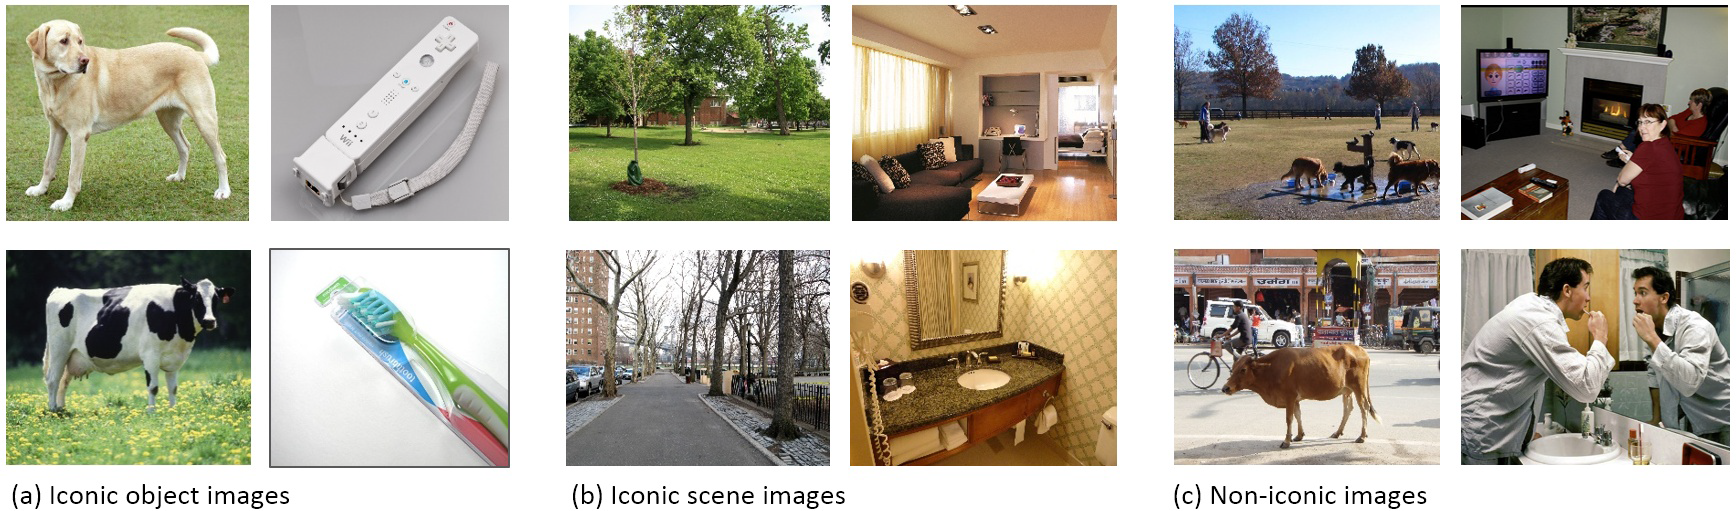
\includegraphics[width=\linewidth]{coco_images.png}
           \end{figure}
\end {itemize}

\end{frame}

\begin{frame}{Datasets}{Flickr30k Entities \cite{Plummer2015}}
\begin{wideitemize}
\item 276.000 annotated bounding boxes 
\item corresponding fragments of captions
\end{wideitemize}
\begin{figure}[tb]
           \centering
           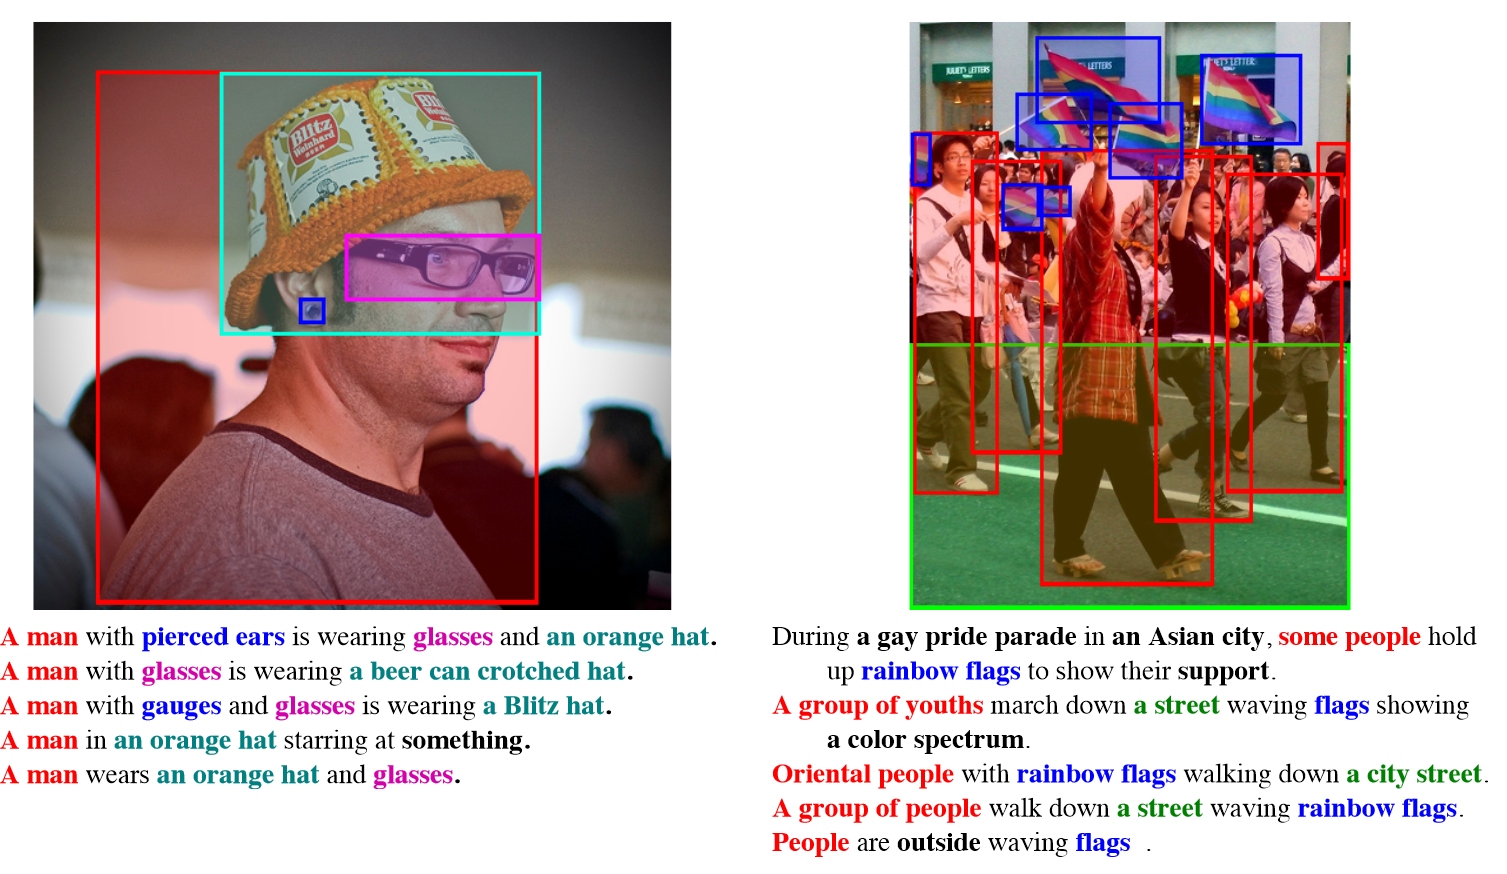
\includegraphics[width=\linewidth]{entities.png}
           \end{figure}

\end{frame}

% cite plummer etc .... 

% ----------------------------------------------------------------------------------

\section{Methodology}%T

\begin{frame}{Methodology}
\begin{wideitemize}
\item modify NeuralTalk code which implements both Karpathy and Vinyals
\item Feedforward Sequential Memory Neural Networks without Recurrent Feedback %ref Zhang
\item LDA
\begin{itemize}
\item learn LDA on training set
\item train perceptron to predict topic distribution on given image feature
\item predict topic distribution on unseen images with network
\item use topic distribution as additional input for RNN
\end{itemize}
\end{wideitemize}
\end{frame}

\begin{frame}{Methodology}
\begin{wideitemize}
\item transform Flickr30kEntities to useful data
\begin{itemize}
\item tf-idf representation for sentence snippets
\item CNN feature vectors for image snippets
\end{itemize}
\item add semantic information with guided LSTM
\begin{itemize}
    \item stacked CCA based on Flickr30kEntities data
    \item LDA
\end{itemize}
\end{wideitemize}
\end{frame}


% ----------------------------------------------------------------------------------

\section{Preliminary Results}%
\begin{frame}{Results from literature}
\begin{table}[]
\centering
\begin{tabular}{lllll}
                  & \textbf{B1} & \textbf{B2} & \textbf{B3} & \textbf{B4} \\ \hline
\textbf{Karpathy} & 57.3        & 36.9        & 24.0        & 15.7             \\
\textbf{Vinyals}  & 66.3        & 42.3        & 27.7        & 18.3        \\
\textbf{Jia}      & 64.4        & 44.6        & 30.5        & 20.6        \\
\textbf{Human}    & 68          &             &             &             \\ \hline
\end{tabular}
\end{table}

\end{frame}
\begin{frame}{Experimental Results}
\begin{table}[]
\centering
\begin{tabular}{lllll}
\multicolumn{1}{c}{}    & \textbf{B1} & \textbf{B2} & \textbf{B3} & \textbf{B4} \\ \hline
\textbf{RNN}       & 65.1        & 43.1        & 29.0        & 18.9        \\
\textbf{RNN + LDA} & 64.5        & 43.1        & 27.9        & 17.6        \\
\textbf{LSTM}        & 59.1        & 37.2        & 22.8        & 14.0        \\
\textbf{Human}          & 68          &             &             &             \\ \hline
\end{tabular}
\end{table}

\end{frame}

\section{Future Work}
\begin{frame}{Future Work}
\begin{wideitemize}
\item finetune current networks
\item finish gLSTM with Flickr30k Entities and LDA
\item investigate dense captioning
\begin{itemize}
    \item Faster RCNN
    \item Flickr30k Entities
\end{itemize}
\item use Torch to make a faster implementation
\end{wideitemize}

\end{frame}
\section{Conclusion}

\begin{frame}{Conclusion}
\begin{wideitemize}
\item working implementations
\item similar/better results are possible
\item new ideas to further investigate
\end{wideitemize}

\end{frame}


\begin{frame}{}
\centering
\Huge{Questions?}
\end{frame}

\scriptsize
\begin{frame}[allowframebreaks]{References}
\bibliographystyle{apalike}
\bibliography{referenties}
\end{frame}


\end{document}


